\documentclass[times, utf8, zavrsni]{fer}
\usepackage{booktabs}


\usepackage[croatian]{babel} 
\usepackage{amssymb}
\usepackage{amsmath}
\usepackage{txfonts}
\usepackage{mathdots}
\usepackage{titlesec}
\usepackage{array}
\usepackage{lastpage}
\usepackage{etoolbox}
\usepackage{tabularray}
\usepackage{color, colortbl}
\usepackage{adjustbox}
\usepackage{geometry}
\usepackage[classicReIm]{kpfonts}
\usepackage{hyperref}
\usepackage{fancyhdr}
\usepackage[T1]{fontenc}     % default is 'OT1'
\usepackage[utf8]{inputenc}
\usepackage{graphicx}

\usepackage{float}
\usepackage{setspace}
\restylefloat{table}


%boja za privatni i udaljeni kljuc u tablicama
\definecolor{LightBlue}{rgb}{0.9,0.9,1}
\definecolor{LightGreen}{rgb}{0.9,1,0.9}

%Promjena teksta za dugačke tablice
\DefTblrTemplate{contfoot-text}{normal}{Nastavljeno na idućoj stranici}
\SetTblrTemplate{contfoot-text}{normal}
\DefTblrTemplate{conthead-text}{normal}{(Nastavljeno)}
\SetTblrTemplate{conthead-text}{normal}
\DefTblrTemplate{middlehead,lasthead}{normal}{Nastavljeno od prethodne stranice}
\SetTblrTemplate{middlehead,lasthead}{normal}


%Programski kod
\usepackage{courier} %% Sets font for listing as Courier.
\usepackage{listings, xcolor}
\lstset{
tabsize = 4, %% set tab space width
showstringspaces = false, %% prevent space marking in strings, string is defined as the text that is generally printed directly to the console
numbers = left, %% display line numbers on the left
commentstyle = \color{green}, %% set comment color
keywordstyle = \color{blue}, %% set keyword color
stringstyle = \color{red}, %% set string color
rulecolor = \color{black}, %% set frame color to avoid being affected by text color
basicstyle = \scriptsize \ttfamily , %% set listing font and size
breaklines = true, %% enable line breaking
numberstyle = \tiny,
}




\begin{document}

% TODO: Navedite broj rada.
\thesisnumber{663}

% TODO: Navedite naslov rada.
\title{Mobilna igra za vježbanje matematike}

% TODO: Navedite vaše ime i prezime.
\author{Denis Pipalović}

\maketitle

% Ispis stranice s napomenom o umetanju izvornika rada. Uklonite naredbu \izvornik ako želite izbaciti tu stranicu.
\izvornik

% Dodavanje zahvale ili prazne stranice. Ako ne želite dodati zahvalu, naredbu ostavite radi prazne stranice.
\zahvala{}

\tableofcontents

\chapter{Uvod}
	Matematika, osim što je predmet koji se predaje u svim razredima osnovnih i srednjih škola, također je i znanost iz područja prirodnih znanosti.
Značaj matematike vidljiv je ne samo u drugim poljima područja prirodnih znanosti, već i u svim drugim područjima, posebice u području tehničkih znanosti.
Ne poznavanje osnova matematike negativno se odražava na učenikove školske uspjehe kroz cijelo školovanje. Jedan od problema svakako je problem pristupa nastavnika
 u učenju matematike, odnosno manjak povlačenja paralela sa stvarnim svijetom i pokazivanja primjena matematike; ovakav pristup demotivira učenika u vježbanju matematike
i savladavanju čak i osnovnih računskih operacija. Jednom izgubljenu motivaciju za neko područje teško je vratiti nazad.

Primjenom gamifikacije u edukaciji učenicima bi se razne teme i ishodi učenja mogle prezentirati kroz zanimljive načine, samim time i povećati zainteresiranost za nekom temom 
ili predmetom. S obzirom na to da djeca u novije doba koriste pametne uređaje sve više i više, gamifikacija jedan od način kroz koji bi to vrijeme na mobitelu moglo biti potrošeno
 u edukativne svrhe; kroz zabavu!

S obzirom na navedeno, tema ovog rada je napraviti mobilnu igru za vježbanje matematike u nižim razredima osnovne škole koja će kroz zanimljiv i interaktivan način pružati  ugodnije iskustvo
vježbanja matematičkih zadataka. Igra je zamišljena kao tzv. „endless runner“ u kojoj igrač skuplja padajuće objekte ovisno o trenutnom zadatku (npr. samo parne brojeve, brojeve veće od zadanog,
brojeve djeljive s određenim brojem, samo kvadrate i slično) i sakuplja bodove. Kako igra ne bi postala monotona kroz kratko vrijeme igranja cilj je napraviti da igra postaje progresivno sve teža
i teža, no do te mjere da se ne postigne negativan efekt u drugom ekstremu; igra ne smije postati niti previše teška jer bi samim time postala i demotivirajuća! Stoga je cilj da se težina igre
dinamički prilagođava mogućnostima učenika. Osim same mobilne igre, potrebno je izgraditi i jednostavno web sučelje za učitelja kako bi mogao postavljati tipove zadataka koji prate temu onoga što
se trenutno predaje na nastavi. Kroz navedeno web sučelje nastavniku će se pružati i mogućnost pregleda rezultata pojedinog učenika te uvid u detalje igre kao što je tip zadatak na kojem je učenik 
griješio, ukupno vrijeme igranja i slično. Kako bi igra bila dostupna svima koji ju požele igrati, odnosno kako igra ne bi ovisila o postavkama učitelja, postojati će i zadane postavke koje će se moći
 prilagođavati kroz postavke same igre. 



\chapter{Naslov 1}
Poglavlje 1

\section{Introduction}
Podpoglavlje 1.1

\section{Introduction}
Podpoglavlje 1.2

\chapter{Implementacija mobilne igre}

	\section{Pozadina}
	Pozadina je tematski zamišljena kao put iz središta zemlje  do dubokog svemira. Mobilna igra je takozvani endless runner, što znači da se potencijalno može igrati beskonačno,
	odnosno ne postoji način na koji igra završava osim u slučaja da igrač izgubi sve živote, stoga je osim samog efekta "putovanja ka svemiru" potrebno osigurati i beskonačno pomicanje same pozadine.
	
	Pozadina kao takva se u konačnici sastoji od 20ak slika čije spajanje vertikalno daje efekt kontinuiranosti. Dok poznati pokretački strojevi (engl. \textit{game engine}) poput Unity nudi opcije manipulacija
	pozadinom, kao što je beskonačno ponavljajuća pozadina, ta mogućnost u ovakvom razvoju aplikacije nije moguća, već ju je potrebno iskodirati samostalno. 
	Za početak je potrebno učitati slike pozadina kao Bitmap te ih omotati u objekte kako bi im se dala različita svojstva poput x i y koordinata gdje se trenutno nalaze. Takvi objekti pohranjeni su u polje.
	
	Radi jednostavnosti, svaka slika pozadine se  vertikalno i horizontalno skalira na broj piksela koje zaslon mobitela ima; zbog toga, u jednom trenutku na zaslonu se mogu vidjeti maksimalno dvije slike
	pozadine od jednom. Na samom početku igre uzimaju se prva dva objekta pozadine iz polja. Prvi objekt predstavlja donju pozadinu koja će biti prikazana, a drugi gornju pozadinu.  Donju pozadinu potrebno je inicijalizirati
	na lokaciju sa x koordinatom 0 i y koordinatom 0, odnosno želimo da se pokazuje od početka zaslona vertikalno i horizontalno. Drugu sliku inicijaliziramo opet tako da joj damo x koordinatu 0, no y koordinatu postavljamo
	na minus vertikalnu veličinu zaslona. Na svako ponovno osvježavanje igre, pozadina se vertikalno spušta ka dolje čime se stvara efekt putovanja igrača prema gore. Spuštanje pozadine prema dolje implementacijski je 
	ostvareno tako što se svakim osvježavanjem zaslona povećava y koordinata obje slike za određenu vrijednost, ovisno o tome kojom brzinom želimo da "igrač putuje ka svemiru". 
	
	Na sljedećoj slici može se vidjeti način iscrtavanja pozadine na ekranu i izvan njega.
	
	\begin{figure}[H]
			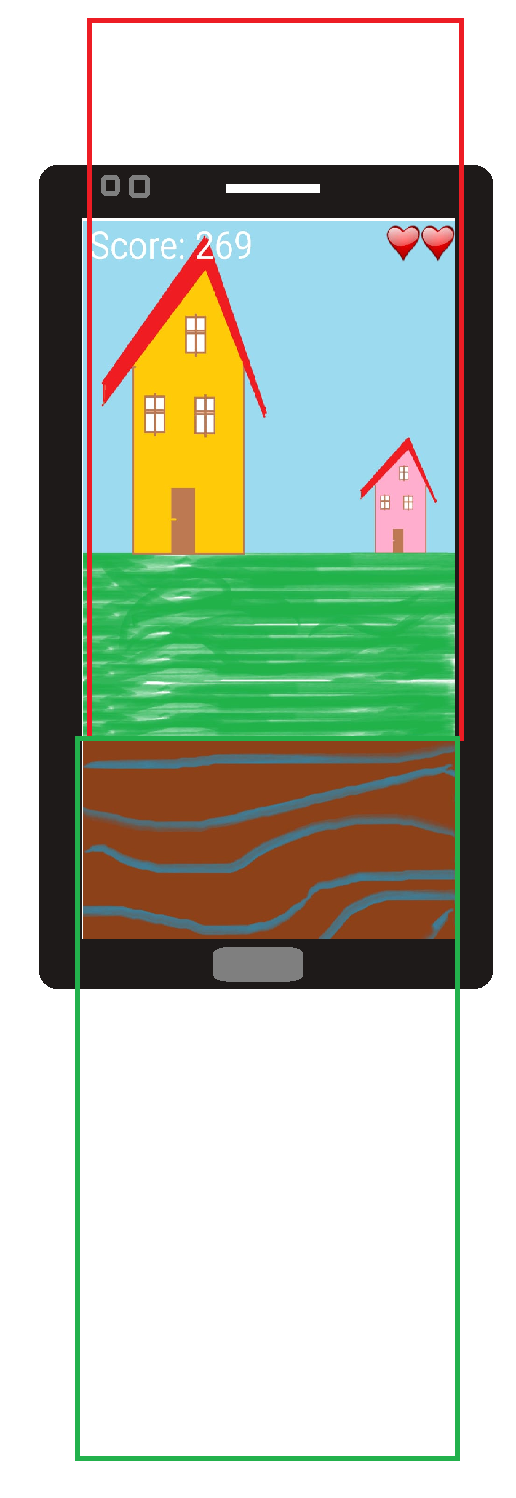
\includegraphics[scale=0.6]{"slike/background.png"} 
			\centering
			\caption{Pomicanje pozadine}
			\label{fig:pomicanjepozadine}
		\end{figure}
		

	
	U trenutku kada y koordinata donje slike izađe izvan ekrana (odnosno kada je vrijednost y osi veća od y dimenzije ekrana) nova donja slika sada je slika koja je bila gore, a novu gornju sliku uzimamo 
	kao sljedeći član polja. 
	Zadnja slika prikazuje svemir pun zvijezdi i nju u polje učitavamo dva puta (dva različita objekta). U trenutku kad smo u igri došli do te slike, tim dvijema slikama se konstanto mijenjaju vrijednosti y osi.
	Odnosno kad donja slika izađe dolje s ekrana, ponovno se postavljaju vrijednosti y osi za obje slike. 
	
	
	Cijeli način implementacije pomicanja pozadine možemo prikazati sljedećim kodom:
	
	\begin{lstlisting}[language = Java , frame = trBL , firstnumber = 1 , escapeinside={(*@}{@*)}]
   private void updateBackground() {
        currentDownBackground.setY(currentDownBackground.getY() + 5);
        currentUpBackground.setY(currentUpBackground.getY() + 5);

        if (currentDownBackground.getY() > screenY) {
            currentDownBackground = currentUpBackground;
            if (currentBackgroundIndex < backgrounds.length - 1)     
                currentUpBackground = backgrounds[++currentBackgroundIndex]; 
            else {
                currentDownBackground = backgrounds[backgrounds.length - 2];
                currentDownBackground.setY(0);
                currentUpBackground = backgrounds[backgrounds.length - 1];
            }
            currentUpBackground.setY(-screenY);
        }
    }
	\end{lstlisting}


	\section{Objekt za skupljanje}
	Slično kao i pozadinu, objekt koji se kontrolira, odnosno objek s kojim se skupljaju padajući objekt učitan je kao kao Bitmap, odnosno više njih, konkretnije kao dva Bitmap objekta omotana sa objektom
	klase "Saw". Za razliku od pozadine koja je putovala prema dolje, objekt s kojim skupljamo padajuće objekte je statičan na ekranu, odnosno ne mijenja svoj položaj na ekranu bez korisničke akcije. Pod kornisničku akciju u 
	ovom slučaju podrazumijeva se dodir ekrana. Koristeći oblikovni obrazac promatrač (engl. \textit{observer}), pri inicijalizaciji igre  subjektu (objektu konkretne klase "View", u ovom slučaju to je "SurfaceView")
	se postavlja konkretna implementacija apstraktnog promatrača "OnTouchListener". Navedeno sučelje sastoji se od jedne funkcije:
	\begin{lstlisting}[language = Java , frame = none , numbers=none, escapeinside={(*@}{@*)}]
		boolean onTouch(View v, MotionEvent event); 
	\end{lstlisting}
	
	Ova funkcija prima dva parametra, "View v" koji je pokazivač na "View" kojem je događaj dodira dostavljen te parametar "MotionEvent event" koji opisuje tip događaja. Primjeri tipova događaja su: 
	"ACTION\_DOWN" koji govori da se dogodio pritisak na zaslonu, "ACTION\_UP" koji govori da je dodir zaslona otpušten, "ACTION\_MOVE" koji govori da se dogodila promjena pozicije između pritiska ("ACTION\_DOWN") i otpuštanja
	("ACTION\_UP") te nekolicina raznih drugih akcija. Navedena funkcija vraća primitivni tip boolean koji u ovom slučaju predstavlja zastavicu koja govori da li je konkretni promatrač "konzumirao događaj do kraja".
	
	U nastavku je prikazan cijeli programski kod potreban za pomicanje objekta za skupljanje. Konkretna implementacija sučelja "OnTouchListener" izvedena je kao anonimni razred, odnosno zbog bolje preglednosti koda 
	koristi se pokrata u vidu lambda izraza, dok "this" predstavlja objekt klase View.

		\begin{lstlisting}[language = Java , frame = trBL , firstnumber = 1 , escapeinside={(*@}{@*)}]
			this.setOnTouchListener((v, event) -> {
				if (event.getAction() == MotionEvent.ACTION_MOVE) {
					saw.setX((int) event.getX());
				}
				return true;
			});
		\end{lstlisting}
		
	Na ovom programskom kodu potrebno je uočiti da se kontroliranje našeg objekta može dogoditi doticanjem i pomicanjem prsta na bilo kojem dijelu ekrana, no da sam objekt kojeg kontroliramo neće promijeniti 
	vrijednost svoje x osi, odnosno neće se pomicati vertikalno, već se isključivo mijenja vrijednost položaja na horizontalnoj osi; također je bitno uočiti da za pomicanje objekta nije potrebno stisnuti na objekt
	te ga povući, već je dovoljno stisnuti na određeno mjesto na ekranu te će se objektov položaj na horizonalnoj osi teleportirati na željeno mjesto. Iako je ovo programsko riješenje vjerojatno najjednostavnije, 
	kasnije će se ispostaviti da je ujedno i najbolje. Ukratko, može se dogoditi da objekt kojeg kontroliramo bude okružen s padajućim objektima koji se ne smiju pokupiti i stoga je ova mogućnost "teleportiranja" poželjna.
	
	
	Kao što je već ranije navedeno, objekt za skupljanje koji se kontrolira ne mijenja svoj položaj na ekranu (bez prethodne akcije korisnika) već je potreba učitavanja više slika, odnosno stvaranja više Bitmap 
	objekata nastala u svrhu stvaranja animacije. Animacija se stvara tako što se brzo izmijenjuju slike koje se iscrtavaju na zaslonu. Konkretno, ova animacija sastoji se od dvije slike koje se neprestano izmijenuju.
	Prva slika nastala je jednostavnim crtanjem, dok je druga nastala rotacijom za određeni kut te dodavanjem dodatnih detalja. 
	
	Sljedeće dvije slike prikazuju objekt s kojim skupljamo padajuće objekte, odnosno zajedno prikazuju oštricu koja se rotira velikom brzinom.
	
	
	
		\begin{figure}[!htb]
			\begin{minipage}{0.48\textwidth}
				\centering
				
\includegraphics[scale=0.6]{"slike/saw1.png"} 
				\caption{Originalna slika oštrice}
				\label{fig:saw1}
			\end{minipage}\hfill
			\begin{minipage}{0.48\textwidth}
				\centering
				
\includegraphics[scale=0.6]{"slike/saw2.png"} 
				\caption{Zarotirana originalna slika oštrice sa dodatnim detaljima}
				\label{fig:saw2}
			\end{minipage}
		\end{figure}
	
	\section{Padajući objekti}

\chapter{Baza podataka}
	Baze podataka su organizirane kolekcija podataka koje omogućavaju laki pristup podacima, uređivanje podataka i upravljanje istih. U sklopu ovog projekta koristio se
	SQL tip baze podataka, konkretnije PostgreSQL. PostgreSQL je besplatni, open-source sustav za upravljanje bazom podataka (SUBP) iza kojeg je više od 30 godina aktivnog razvoja.
	
	
	\section{ER dijagram}
		Sljedeća slika prikazuje ER dijagram baze podataka.
		\begin{figure}[H]
			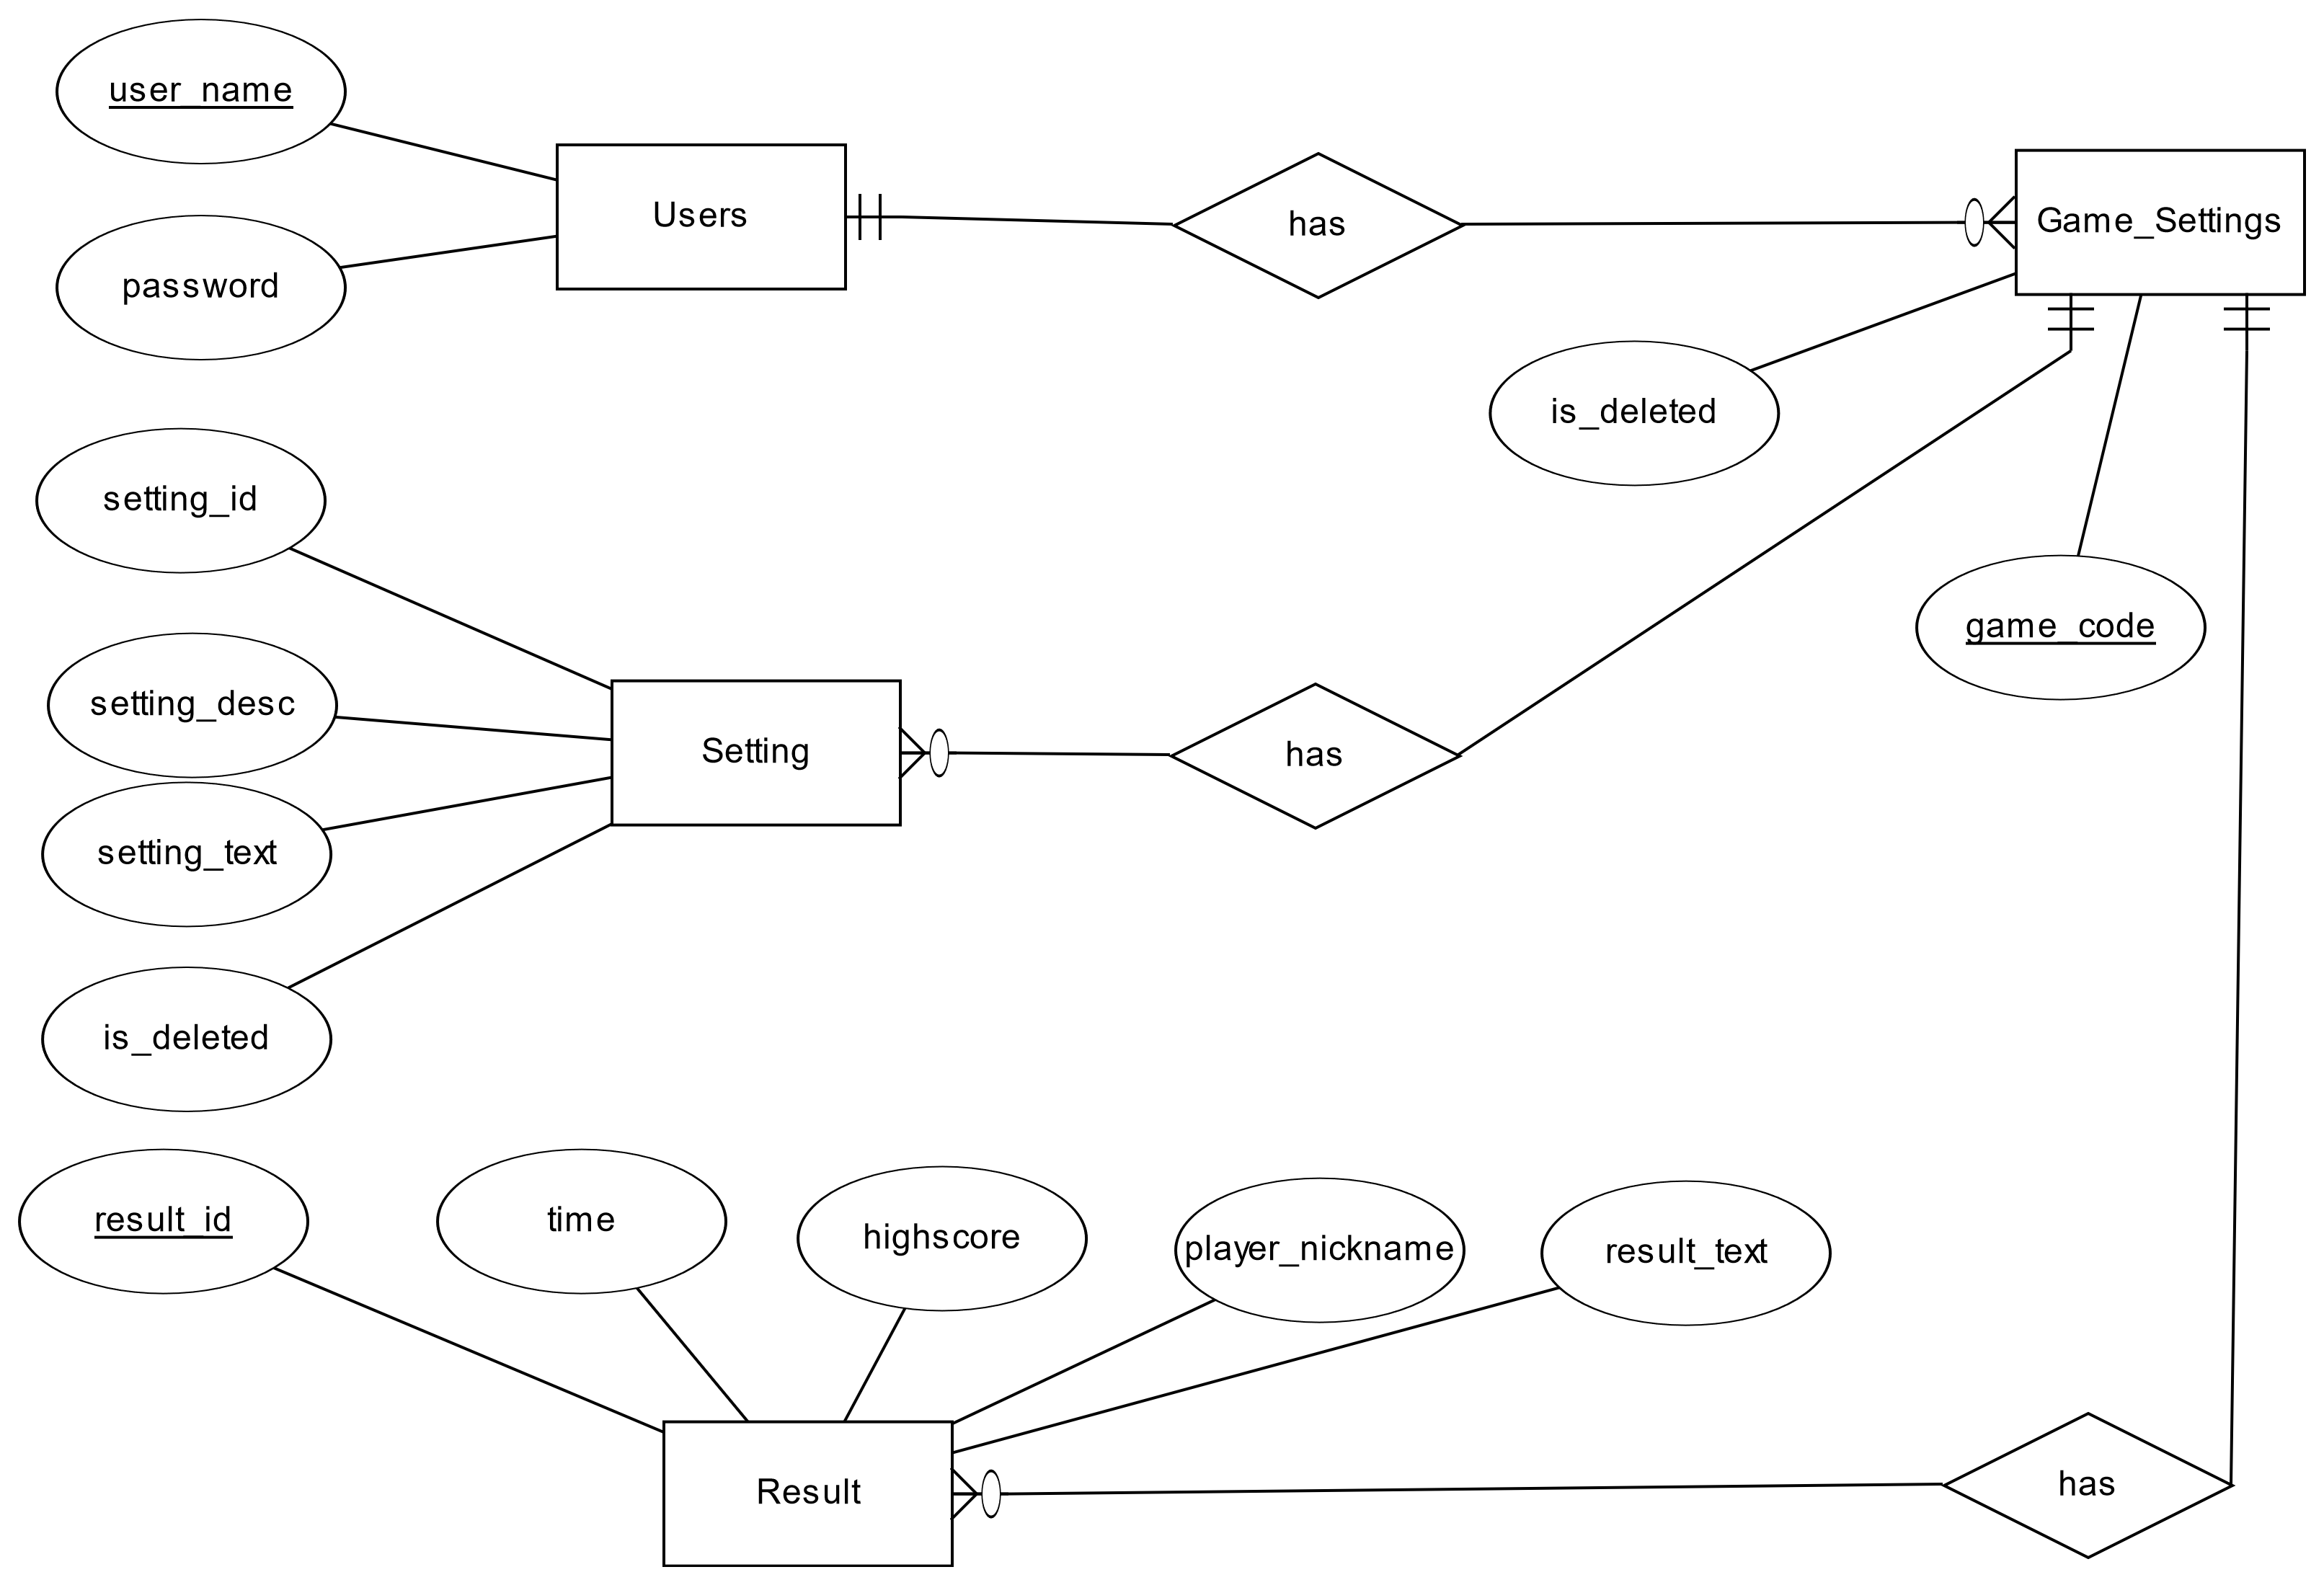
\includegraphics[width=\linewidth]{"slike/ER.png"} 
			\centering
			\caption{ER dijagram baze podataka}
			\label{fig:erdijagram}
		\end{figure}

	
	\section{Opis entiteta i tablica}
			\textbf {Users} \hspace{5mm}
			{Ovaj entitet označava korisnika koji koristi web aplikaciju, odnosno web sučelje za učitelja. Sadrži atribute: user\_ name i password.
			Atribut user\_ name predstavlja korisničko ime korisnika, dok atribut password označava zaporku koja se ne sprema u "plain-textu", već kao 
			rezultat hash funkcije.
			Ovaj entitet u vezi je \textit{One-To-Many} s entitetom Game\_ Settings preko atributa user\_name.}
				
				\begin{longtblr}[
					label=none,
					entry=none
					]{
						width = \textwidth,
						colspec={|X[6,l]|X[6, l]|X[20, l]|}, 
						rowhead = 1,
					} %definicija širine tablice, širine stupaca, poravnanje i broja redaka naslova tablice
					\hline \multicolumn{3}{|c|}{\textbf{Users}}	 \\ \hline[3pt]
					\SetCell{LightGreen}user\_name & VARCHAR	&  	jedinstveni naziv korisnika  	\\ \hline
					password	& VARCHAR &  rezultat hash funkcije nad zaporkom 	\\ \hline 
				\end{longtblr}



			\textbf {Game\_ Settings} \hspace{5mm}
			{Ovaj entitet označava jedan "game room". Sadrži atribute: game\_ code i is\_ deleted.
			Ovaj entitet u vezi je \textit{Many-To-One} s entitetom Users preko atributa user\_ name, u vezi \textit{One-To-Many} s
			entitetom Setting preko atributa game\_ code te u vezi \textit{One-To-Many} s entitetom Result preko atributa game\_ code.}
				
				\begin{longtblr}[
					label=none,
					entry=none
					]{
						width = \textwidth,
						colspec={|X[6,l]|X[6, l]|X[20, l]|}, 
						rowhead = 1,
					} 
					\hline \multicolumn{3}{|c|}{\textbf{Game\_ Settings}}	 \\ \hline[3pt]
					\SetCell{LightGreen}game\_ code & INT	&  	jedinstveni idenfitikator game\_ settings   	\\ \hline
					is\_ deleted & INT & zastavica koja govori jesu li "game room" obrisan \\ \hline
					\SetCell{LightBlue}user\_ name & VARCHAR & oznaka korisnika kojem "game room" pripada \\ \hline
				\end{longtblr}


			\textbf {Setting} \hspace{5mm}
			{Ovaj entitet označava jedanu postavku. Sadrži atribute: setting\_ id, setting\_ desc, setting\_ text i is\_ deleted.
			Ovaj entitet u vezi je \textit{Many-To-One} s entitetom Game\_ Settings preko atributa game\_ code.}
				
				\begin{longtblr}[
					label=none,
					entry=none
					]{
						width = \textwidth,
						colspec={|X[6,l]|X[6, l]|X[20, l]|}, 
						rowhead = 1,
					} 
					\hline \multicolumn{3}{|c|}{\textbf{Setting}}	 \\ \hline[3pt]
					\SetCell{LightGreen}setting\_ id & INT	&  	jedinstveni idenfitikator za Setting  	\\ \hline
					setting\_desc & VARCHAR & tekst koji opisuje cilj zadatka \\ \hline
					setting\_text & VARCHAR & postavka formatirana tako da bude razumljiva mobilnoj igri \\ \hline
					is\_ deleted & INT & zastavica koja govori je li postavka obrisana \\ \hline
					\SetCell{LightBlue}game\_code & INT & oznaka Game\_Settings kojem Setting pripada \\ \hline
					
				\end{longtblr}
				
			
			\textbf {Result} \hspace{5mm}
			{Ovaj entitet označava jedan rezultat igranja igre na mobitelu uz preuzete postavke.
			Sadrži atribute: result\_ id, time, highscore, player\_ nickname te result\_ text.
			Ovaj entitet u vezi je \textit{Many-To-One} s entitetom Game\_ Settings preko atributa game\_ code.}
				
				\begin{longtblr}[
					label=none,
					entry=none
					]{
						width = \textwidth,
						colspec={|X[6,l]|X[6, l]|X[20, l]|}, 
						rowhead = 1,
					} 
					\hline \multicolumn{3}{|c|}{\textbf{Result}}	 \\ \hline[3pt]
					\SetCell{LightGreen}result\_ id & INT	&  	jedinstveni idenfitikator za Result  	\\ \hline
					time & VARCHAR & vrijeme pohrane rezultata u bazu podatka \\ \hline
					highscore & VARCHAR & ostvareni rezultat na igri  \\ \hline
					player\_ nickname & VARCHAR & nadimak igrača  \\ \hline
					result\_text & VARCHAR & JSON polje s događajima igre  \\ \hline
					\SetCell{LightBlue}game\_code & INT & oznaka Game\_Settings kojem Result pripada \\ \hline
					
				\end{longtblr}

	\newpage
	\section{Relacijski dijagram}
		Sljedeća slika prikazuje relacijski dijagram baze podataka.
		\begin{figure}[H]
			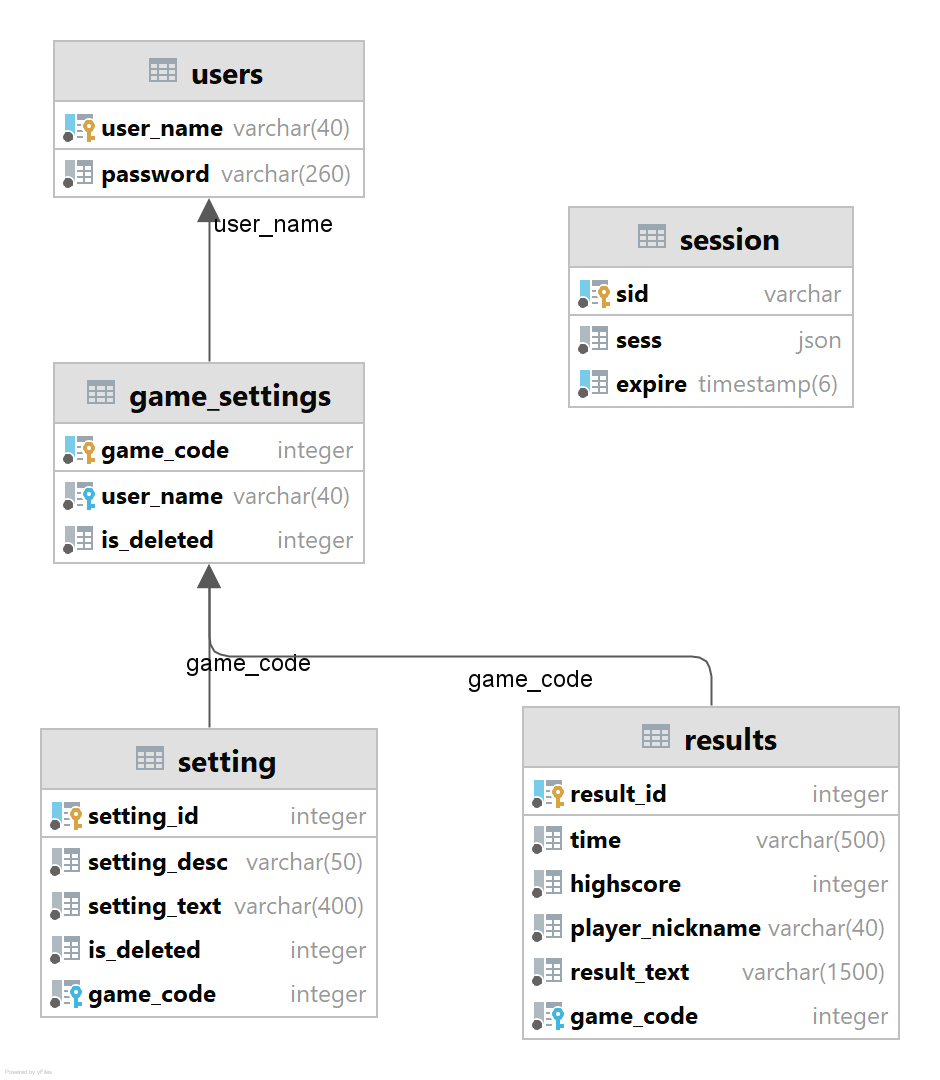
\includegraphics[width=\linewidth]{"slike/REL.png"} 
			\centering
			\caption{Relacijska shema baze podataka}
			\label{fig:relshema}
		\end{figure}


\chapter{Naslov 4}
Poglavlje 4

\bibliography{literatura}
\bibliographystyle{fer}

\begin{sazetak}
Sažetak na hrvatskom jeziku.

\kljucnerijeci{Ključne riječi, odvojene zarezima.}
\end{sazetak}

% TODO: Navedite naslov na engleskom jeziku.
\engtitle{Mobile game for practicing math}
\begin{abstract}
Abstract.

\keywords{Keywords.}
\end{abstract}

\end{document}
